\section{Løsning til speckle pattern robot} \label{Produkt}
Produktet der ses i figur \ref{fig: CAD full assembly}, er den endelige løsning.

\begin{figure}[H]
    \centering
    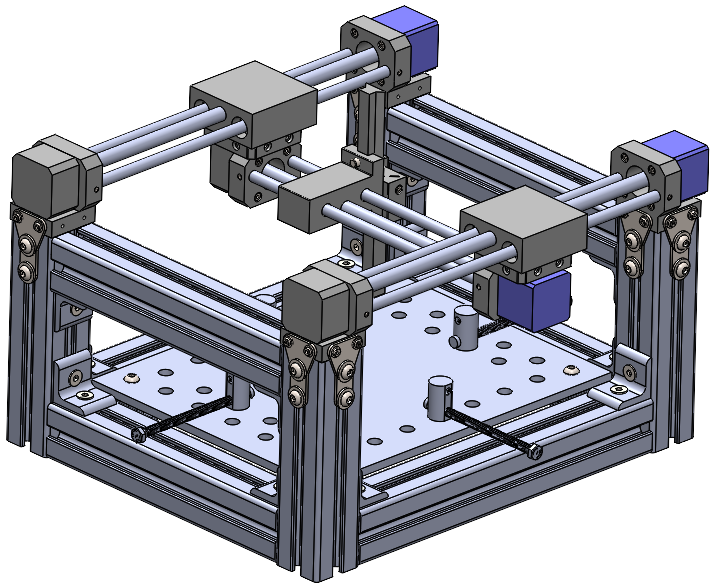
\includegraphics[width=0.7\linewidth]{Sections/6 Detaljeløsning/Media/final assembly.png}
    \caption{Illustration af løsning, med markering af vigtigste dele}
    \label{fig: CAD full assembly}
\end{figure} \plainbreak{-1}


Løsningen fungerer ved, at emnet placeres på arbejdspladen, hvorefter emnet manuelt indspændes. Bevægelsen på x-aksen drives af en motor, som roterer en ledeskrue, hvorpå der bevæges en vogn frem og tilbage og understøttet af følgestænger. Motorerne som driver x-aksen og ledeskruerne, er monteret til en indspændingsblok, som sørger for at følgestængerne fastholdes. Indspændingsblokken er fast monteret til et stel. Stellet består af en kombination af aluminium ekstruderet t-slots i forskellige længder. I ledeskruernes modsatte ende sidder yderligere en indspændingsblok, som både fastspænder følgestængerne og indeholder et kugleleje til ledeskruen. For at opnå bevægelse på y-aksen, er der monteret en motor på x-aksens ene vogn og en kontra vægt på den anden vogn. Mellem de to vogne udspændes yderligere en ledeskrue og to følgestænger, som driver en vogn, der har PeJV'en monteret. Vognen på y-aksen er udformet så PeJV'en kan justeres manuelt i højden, for at passe til forskellige emnehøjder. 



 

